\documentclass[12pt]{article}
\usepackage[margin=1in]{geometry}
\usepackage{amsmath,amsfonts,amssymb}
\usepackage{graphicx}
\usepackage{booktabs}
\usepackage{longtable}
\usepackage{pdflscape}
\usepackage{rotating}
\usepackage{caption}
\usepackage{subcaption}
\usepackage{setspace}
\usepackage{hyperref}
\usepackage{float}
\usepackage{array}
\usepackage{multirow}
\usepackage{threeparttable}
\usepackage{rotating}
\usepackage{comment}
\usepackage[backend=biber, style=authoryear, natbib]{biblatex}
\usepackage{booktabs}
\usepackage{setspace}
\addbibresource{casino.bib} 
\renewcommand*{\nameyeardelim}{\addcomma\addspace}

% Custom commands for better table formatting
\newcommand{\specialcell}[2][c]{%
  \begin{tabular}[#1]{@{}c@{}}#2\end{tabular}}

\title{The Destruction of Social Capital and Family Flight: Evidence from Casino Openings}
\author{Malcolm Kass\thanks{University of Dallas, Department of Economics. Email: mkass@udallas.edu} \and John Soriano\thanks{University of Dallas, Department of Economics. Email: jsoriano@udallas.edu}}
\date{\today}

\begin{document}

\maketitle

\begin{abstract}
IN PROGRESS, DO NOT CITE: Casino development is often promoted as an engine of local economic growth, but its broader social consequences remain less understood. This paper investigates how casino openings reshape demographic patterns and family-supporting institutions in U.S. counties from 2003 to 2023. Exploiting staggered treatment timing in a difference-in-differences framework, we document consistent evidence that casinos erode community structures. We estimate a 1.28 percentage point decline in fertility rates for women, tied to an estimated drop of 55 children per 1000 women and 26 children per 1000 men. These effects are not a result of new movers to the community where a new casino opened. These demographic shifts are mirrored in weakened religious institutions: religious adherence declines by an estimated 9.5 percentage points, particularly in Catholic communities. The results demonstrate that casinos generate possible social capital losses alongside their economic activity, altering the composition of local populations and undermining religious institutions historically central to family and community life.
\end{abstract}

\begin{comment}
This paper examines the effects of casino openings on family formation and community institutions using a differences-in-differences design with staggered casino openings across U.S. counties from 2000-2023. We find that casinos systematically reduce fertility and disrupt family-supporting institutions through both behavioral change among long-term residents and selective migration. Population declines are concentrated among children and child-rearing age adults, while religious adherence and school enrollment also decline significantly.
\end{comment}
\newpage

\section{Introduction}

\doublespacing
%Kass:  Global vs. Local effects of casinos

Local community officials often credit new casinos as significant economic drivers, which in turn promote economic inflows into the local area because of the new entity. \parencite{keranews2025irvingcasino} However, negative attention has come to light regarding the effects of gambling on local communities. While generating some economic benefits, often stemming from localized increases in employment and tax revenues, evidence is accumulating of the negative spillovers of gambling on the social strata of local communities. These effects are often aceberated due to the addictive nature of risky gambling behavior, esp for lower income households, where researchers estimate that, since the advent of online gambling, only 4\% of individuals earn income and 5.3\% gamble more than 10\% of their monthly income. And these effects are often exacerbated by the addictive nature of gambling, in patiticular harming lower income individuals, households with families, and possible feritility. \parencite{Clark2024LegalizedGambling}  Gambling may be paticularly concerning to officials because of gambling effect of population growth. Local communities may wish to promote in-bound migration into a community and along with fertility as sources of this growth . Hence, researchers need to determine whether industries, such as gambling, generate these negative effects on community and family formation, including fertility. 


Our interests with the effects of casinos are two-fold. First, motivated by the current situtation with a potential casino resort by our institution, we focus on tabla rasa situtations, where a casino resort first moves into a new community without a previous casino presence. Hence our data of interest are different from the "entertainment district" situtations where the economic theory may be unclear on the magnitude of possible outcomes.  Diminshing returns predicts larger effect magnitudes for these first mover casinos, but the possibility of negative network externalities may aceberate the social ills of casinos. Second, and more importantly to the authors' perspective, the effects of casinos on family formation and fertility as well as on community institutions, such as schools and religious institutions, appear to be understudied in the reserach. Casinos represent a significant change to local communities, yet their effects on family formation and community institutions, and the corresponding heterogenieties in the effects across communities, remain relatively unexplored. Current reserch either relies on descriptive event analysis studies that focus on one regions or lack key covariates that may limit coefficient precision. \parencite{moellman2013indian,stitt2003does}  

We constructed a specialized dataset of casino openings across the United States matched to American Community Survey (ACS) microdata from 2000-2023 for family formation outcomes, Religious Congregations \& Membership Studies data from 2000, 2010, and 2020 for religious adherence, and casino opening data covering 11 casino counties with staggered Difference in Difference treatment timing. We find that the presence of a first mover casino harm the trajectories of population growth overall, but paticularly decreases in population growth for young and school-age children. We do not find changes in age-adjusted marial rates for women, nor any changes in the likelihood of parenthood, but we do find a 3.1\% decrease in the number of children. Men are 1.1\% less likely to become parents and have 3.5\% less children.   This paper provides the first comprehensive analysis of how casino openings affect marriage, fertility, population composition, and family-supporting institutions using quasi-experimental variation from staggered casino openings across U.S. counties. 


% Our analysis reveals three key findings. (clearly need to update as we move ahead) First, casinos reduce fertility by approximately 5.5\% for women and 2.6\% for men while having minimal effects on marriage rates. Second, the effects operate through selective out-migration of family-oriented residents, with long-term residents showing immediate fertility declines of 5.5-7.3\% at casino opening, suggesting that established families with more children leave casino counties. Third, casinos weaken family-supporting institutions, reducing school enrollment by up to 6.4\% and religious adherence by 35-37 adherents per 1,000 population in medium-religiosity counties.

\section{Background}

\subsection{Economic activity and Family and Community Formation Structures}
We define factors that contribute to family structures as marriage/cohabitation formations and fertilitiy rates. Community structures are defined as insitutions that form social capital.  These included family particiption in formal public and private education instutions and religious instutions. Key in this paper is why the presence of a new casino in an area would affect communitiy and family formation structures. 

Scholars find 'a number of economic changes tied to new economic activity that may contribute to family formation and fertility.  These include incomes, property values, employment level, and wages. Looking at fertility thru the lens of consumptions,  scholars find that positive income shocks drive fertility, with findings ranging from North Dakota's Natural Gas boom  \parencite{kearney2018male} to commodity shocks driving fertility in oil rich areas of Chile. \parencite{gallego2023baby} With this evidence, scholars speculate that the income effect of these shocks overwhelms a possible negative substitution effect due to an increase in the opportunity cost of fertility. Look at the lens of fertility as investment, contrary to historical trends, increases in income increase the marginal propensity to save, which parents may view children as a way to smooth future consumption. \parencite{goldin2021career,doepke2023economics}  

\subsection{Casinos and Economic and Social Outcomes}

Previous work finds that retail property values and local employment, with positive spillovers to the surronding areas have increased. \parencite{wiley2011casino} \footnote{Others find employment increases, but not an improvement in wages. \parencite{cotti2008effect}} Others find these employment benefits, unsurprisingly, centered around hospitality and service industries. \parencite{humphreys2013new} However, these benefits often don't overwhelm the negative externalities on social behaviors, such as crime, because of a casino's presence.\parencite{Soriano2025Why} \parencite{Scavette2022Casinos} Mustard et al (2006) is the seminal paper on this topic. Casino generated crime does not happen immediately, but after a lag of 3-4 years, they estimate an 8\% increase in crime in casino location counties. \parencite{grinols2006casinos}

Casinos may be viewed as a significant change to local communities, with uncertain effects on family formation and community institutions.  Casinos has been found to increase tax revenues, employment, earnings and property values. A number of papers find increases in local tax revenues and local economic activity. \parencite{humphreys2013new,wiley2011casino} However, many of these benefits found in the previous literature appear to be only a step-wise increase in growth, and with limited spillovers only to the hospitality and service industries. \footnote{The entertainment and tourism industries stuggle to build from their capital investment for once the venue is established, it is difficult to expand production of gaming with new capital investments, as compared to manufacturing and other industries.} Others find that casinos do not materialize in today's entertainment saturated environment due to the indability of casinos to generate new spending into a community as compared to substitution spending to the casino from other local entertainment venues. \parencite{scavette2022casinos,Krutz2022Casinos} Casinos have been found to increase employment, with mixed evidence on wages \parencite{cotti2008effect}  Lastly, reserach has found that casinos can also increase property values for local retail businesses in the vicinity of the casino and when casinos are located in a larger entertainment district. \parencite{wiley2011casino} 

Nonetheless, outside of some isolated cases of community welfare improvements in rural areas, \parencite{moellman2013indian}, there is an array of research finding that casinos generate negative externalities on local communities, primarily crime. The seminal paper in this regard is Grinols et al. (2006) \parencite{grinols2006casinos} who find that casinos generate a 8.6\% increase in property crime and a 12.6\% increase in violent crime in casino location counties.  This increase does not happen immediately, but after a lag of 3-4 years. Mechanisms involved are that casinos generate a high concentration of easy targets, people holding significant amount of cash and are located in a concentrated area as well as impoversing the lower income segments of society.  This is exacerbated due to the increasing high stakes gamblind by low income populations due to the presence of legalized gambling. \parencite{Clark2024LegalizedGambling}  Outside of financial considerations, regarding to the gaming activity itself,  gambling as a form of entertainment may cause some substitution effect for parents, substituting away from family time and activities. 

\subsection{Impact of incomes, property values, and crime shocks on family and community formation}

A number of studies find effects of income shocks on fertility decisions. Kearney et al (2018) find that the positive income shocks of the natural gas boom in North Dakota drove a 1.28\% increase in fertility rates, espeically for fathers. \parencite{kearney2018male} Other studies find that commodity shocks, such as the oil boom in Texas, drive fertility rates. \parencite{gallego2023baby} Income matters for fertility, and theory provides mixed results on the direction. Income shocks only only generate the more obvious positive income effect for normal goods, but with a given increase in incomes and wages for an overall area, but these shocks also changes the opportunity costs of effort involved in family formation.  When viewing families and community as a consuption good, people was substition out of family and community formation to take advantage of higher opportunity costs. Family and community formation as savings/investment goods to smooth consumption would mean that increases in income would potentially lower the Marginal Propersity to Consume. Higher income families may view childrn as an investment venue.  \parencite{doepke2023economics,goldin2021career}

Cohabitation and marriage depend on available resources, not only including incomes, but also  time, if this constraint is depleated by partner presence in the household. This is particularly important for families with children, given the importance of the partnership as a coordinating and a risk mitigation struction with pooled resources. Hence, while decreases in incomes and crime are more obvious conerns, time substitution to gaming from childrearing activities may compound and delay family formation. Or may cause out-miggration of families to increase the transaction costs of gaming.

\subsection{Mapping fertility and social capital to communitiy and family formation preferences}

Given the strong social norms tied to family and community formation, one may wonder when these choice are true indictative of preferences or are a another violation of the weak axiom of revealed preference due to strong social norms. \parencite{sen1973behaviour} However, evidence suggests that these behavior are strongly correlated to stated preferences. \parencite{muller2022illusion} 

\section{Data and Summary Statistics}
\subsection{Dependent variables of interest: Demographics and Family formation}

Our analysis combines several datasets to examine casino effects across multiple domains. We use American Community Survey (ACS) microdata from 2000-2023 for family formation outcomes, Religious Congregations \& Membership Studies data from 2000, 2010, and 2020 for religious adherence, and casino opening data covering 68 casino counties with staggered treatment timing.

Table \ref{tab:summary} presents summary statistics by county type. Notable differences emerge: casino counties have lower marriage rates (31.3\% vs 37.9\% in control counties), fewer children per person (0.70 vs 0.82), and different demographic composition with higher Hispanic representation (28.7\% vs 17.8\%) and lower white representation (57.5\% vs 70.7\%), supporting the need for our difference-in-differences identification strategy.

\subsection{Staggered Treatment Variable: New casino startups}

Central to this work was constructing a dataset of casino openings, including the state and county fips codes to merge with our larger ACS dataset. There were multiple sources for this data, many of which involved scouring, including a website called World Casino News, which was the initial source of information. \parencite{WorldCasinoNews_CasinoOpenings} \footnote{\url{https://news.worldcasinodirectory.com/in-the-news/casino-news/casino-openings}}  With this information, we denoted the state and county as well as the adjacent counties to give our data a donut structure, where the treatment is the casino county and when it happened, and where nearby counties are identified, while other, further-out counties will be our control.  In addition, casino or adjacent counties with preexisting casinos before 2003 were excluded from the analysis. In this 2003-2023 time span, there were xxx casino openings in that span for a total of xxx observations of casino and near counties 

However, the current form of our treatment variable would not be in accordance with our main research question. Our central research questions concern a casino location in a tabla rasa situtation, the estimated average population-weighted effect of a singular casino entering a new community with no previous presence of a casino in the area. \footnote{or future presence to obtain clean estimates of this tabla rasa effect}  Therefore, we do not want contamination from new casino counties with previously existing casinos or near counties with previous casinos in relatively close proximity.\footnote{As an example, Clark county in Nevada opened 16 casinos due that time frame}  Hence this reduced our viable new casinos to 11 casino counties with new openings and 57 nearby, adjacent casino counties, and 388 control counties from 2003 - 2023.\footnote{Special thanks to Kim Burch, Grace Bason, and Luke Gonzales for their assistance creating this dataset} 

\subsection{Key control variables}

Confounds we are accounting for include:

%These county numbers are from tabbing the sample_type variable 





% Table 1: Summary Statistics - Input directly without wrapper
\begin{table}[htbp]\centering
\def\sym#1{\ifmmode^{#1}\else\(^{#1}\)\fi}
\caption{Summary Statistics by County Type}
\label{tab:summary}
\begin{tabular}{l*{3}{cc}}
\hline\hline
            &\multicolumn{2}{c}{(1)}  &\multicolumn{2}{c}{(2)}  &\multicolumn{2}{c}{(3)}  \\
            &\multicolumn{2}{c}{Casino Counties}&\multicolumn{2}{c}{Nearby Counties}&\multicolumn{2}{c}{Control Counties}\\
            &        mean&          sd&        mean&          sd&        mean&          sd\\
\hline
married     &       0.313&       0.464&       0.343&       0.475&       0.379&       0.485\\
has\_children&       0.347&       0.476&       0.368&       0.482&       0.409&       0.492\\
num\_children&       0.701&       1.142&       0.740&       1.153&       0.823&       1.186\\
female      &       0.496&       0.500&       0.495&       0.500&       0.495&       0.500\\
age         &      29.086&       6.558&      29.031&       6.636&      29.042&       6.685\\
white       &       0.575&       0.494&       0.666&       0.472&       0.707&       0.455\\
black       &       0.157&       0.364&       0.120&       0.325&       0.131&       0.338\\
hispanic    &       0.287&       0.452&       0.209&       0.407&       0.178&       0.382\\
\hline
\(N\)       &     3305201&            &     2491622&            &    16503448&            \\
\hline\hline
\multicolumn{7}{l}{\footnotesize Notes: Individual-level statistics weighted by person weights. Sample includes individuals aged 18-40.}\\
\end{tabular}
\end{table}


\section{Empirical Strategy}



\subsection{Two-Way Fixed Effects}

We begin with a standard two-way fixed effects (TWFE) specification:

\begin{equation}
Y_{ct} = \alpha + \beta \cdot \text{Post}_{ct} + \mathbf{X}_{ct}'\gamma + \mu_c + \lambda_t + \varepsilon_{ct}
\end{equation}

\noindent where $Y_{ct}$ is the average number of children for women in county $c$ and year $t$, $\text{Post}_{ct}$ is an indicator equal to one if county $c$ has an operating casino in year $t$, $\mathbf{X}_{ct}$ includes demographic controls (average age and age squared), $\mu_c$ are county fixed effects, $\lambda_t$ are year fixed effects, and $\varepsilon_{ct}$ is the error term. We cluster standard errors at the county level and weight by population.

\subsection{Callaway and Sant'Anna Method}

Given concerns about treatment effect heterogeneity and staggered treatment timing, we implement the \parencite{callaway2021difference} approach. This method addresses potential bias in TWFE estimators when treatment effects vary across units or over time.

The CS estimator constructs group-time specific treatment effects $ATT(g,t)$ for cohort $g$ (year of first treatment) in period $t$:

\begin{equation}
ATT(g,t) = E[Y_t(g) - Y_t(0) | G = g]
\end{equation}

\noindent where $Y_t(g)$ is the potential outcome under treatment and $Y_t(0)$ is the potential outcome under control. The method aggregates these group-time effects into an overall average treatment effect on the treated (ATT):

\begin{equation}
ATT = \sum_{g} \sum_{t} w(g,t) \cdot ATT(g,t)
\end{equation}

\noindent where $w(g,t)$ are weights based on group sizes.

We implement the doubly robust (DRIPW) estimator, which combines inverse probability weighting with outcome regression to improve efficiency and robustness. Counties that opened casinos before 2005 are excluded from the CS analysis as ``always treated'' units.

\subsection{Robustness Checks}

To address potential confounding from county-specific trends, we estimate specifications with county-specific linear time trends:

\begin{equation}
Y_{ct} = \alpha + \beta \cdot \text{Post}_{ct} + \mathbf{X}_{ct}'\gamma + \delta_c \cdot t + \mu_c + \lambda_t + \varepsilon_{ct}
\end{equation}

\noindent where $\delta_c \cdot t$ captures county-specific linear trends.

For the CS approach, we include county-specific trends as additional covariates in the outcome regression, allowing the method to condition on these trends when constructing treatment effect estimates.

\subsection{Identification Strategy}

Our identification relies on the assumption that, conditional on controls and fixed effects, the timing of casino openings is quasi-random with respect to fertility trends. While casino placement is endogenous to economic conditions, we argue that the specific timing of openings—often determined by lengthy regulatory processes, ballot initiatives, and legal challenges—provides plausibly exogenous variation in treatment timing.

The key identifying assumption is parallel trends: absent casino openings, treated and control counties would have experienced similar fertility trajectories. We assess this assumption through event study analyses and examine robustness to alternative control group definitions and trend specifications.

\section{Population Effects}
We begin by documenting population effects across age groups. Table \ref{tab:population} shows event study results for log population by age group using our 8-year specification. The effects are substantial and persistent: by 8+ years post-opening, total population declines by 4.4\%, child-rearing age population (18-40) shows minimal decline of 1.4\%, children ($\le$17) decline by 5.7\%, and school-age population (5-17) falls by 6.6\%. The stronger effects on children relative to adults suggests that family formation rather than general population decline is the primary mechanism.

% Table 2: Population Effects - Input directly without wrapper
\begin{table}[htbp]\centering
\def\sym#1{\ifmmode^{#1}\else\(^{#1}\)\fi}
\caption{Population Effects by Age Group}
\begin{tabular}{l*{4}{c}}
\hline\hline
            &\multicolumn{1}{c}{Total Pop}&\multicolumn{1}{c}{Child-Rearing}&\multicolumn{1}{c}{Children}&\multicolumn{1}{c}{School-Age}\\\cmidrule(lr){2-2}\cmidrule(lr){3-3}\cmidrule(lr){4-4}\cmidrule(lr){5-5}
            &\multicolumn{1}{c}{(1)}&\multicolumn{1}{c}{(2)}&\multicolumn{1}{c}{(3)}&\multicolumn{1}{c}{(4)}\\
            &\multicolumn{1}{c}{ln\_total\_pop}&\multicolumn{1}{c}{ln\_child\_rearing\_pop}&\multicolumn{1}{c}{ln\_children\_pop}&\multicolumn{1}{c}{ln\_school\_age\_pop}\\
\hline
t-3         &      -0.042\sym{**} &      -0.032\sym{*}  &      -0.055\sym{***}&      -0.059\sym{***}\\
            &     (0.017)         &     (0.018)         &     (0.021)         &     (0.022)         \\
[1em]
t-2         &       0.010\sym{*}  &       0.002         &       0.015         &       0.017\sym{*}  \\
            &     (0.006)         &     (0.013)         &     (0.009)         &     (0.010)         \\
[1em]
t           &       0.002         &      -0.005         &      -0.009         &      -0.009         \\
            &     (0.006)         &     (0.012)         &     (0.009)         &     (0.009)         \\
[1em]
t+1         &      -0.011         &      -0.015         &      -0.014         &      -0.014         \\
            &     (0.009)         &     (0.015)         &     (0.012)         &     (0.012)         \\
[1em]
t+2         &      -0.021\sym{**} &      -0.011         &      -0.026\sym{*}  &      -0.025\sym{*}  \\
            &     (0.009)         &     (0.013)         &     (0.013)         &     (0.014)         \\
[1em]
t+3         &      -0.023\sym{**} &      -0.003         &      -0.027\sym{*}  &      -0.033\sym{**} \\
            &     (0.012)         &     (0.017)         &     (0.016)         &     (0.016)         \\
[1em]
t+4         &      -0.026\sym{**} &      -0.009         &      -0.033\sym{**} &      -0.038\sym{**} \\
            &     (0.013)         &     (0.017)         &     (0.017)         &     (0.017)         \\
[1em]
t+5         &      -0.029\sym{**} &      -0.017         &      -0.039\sym{**} &      -0.043\sym{**} \\
            &     (0.013)         &     (0.019)         &     (0.017)         &     (0.018)         \\
[1em]
t+6         &      -0.031\sym{**} &      -0.016         &      -0.047\sym{**} &      -0.051\sym{**} \\
            &     (0.015)         &     (0.021)         &     (0.019)         &     (0.020)         \\
[1em]
t+7         &      -0.038\sym{**} &      -0.019         &      -0.050\sym{**} &      -0.052\sym{**} \\
            &     (0.015)         &     (0.021)         &     (0.020)         &     (0.021)         \\
[1em]
t+8+        &      -0.030         &      -0.003         &      -0.040\sym{*}  &      -0.046\sym{*}  \\
            &     (0.020)         &     (0.024)         &     (0.024)         &     (0.026)         \\
\hline
Observations&       6,686         &       6,686         &       6,686         &       6,686         \\
R-squared   &       0.993         &       0.991         &       0.992         &       0.991         \\
\hline\hline
\multicolumn{5}{l}{\footnotesize Standard errors in parentheses}\\
\multicolumn{5}{l}{\footnotesize Standard errors clustered at county level in parentheses.}\\
\multicolumn{5}{l}{\footnotesize Donut sample excludes nearby counties. All variables in logs.}\\
\multicolumn{5}{l}{\footnotesize \sym{*} \(p<0.10\), \sym{**} \(p<0.05\), \sym{***} \(p<0.01\)}\\
\end{tabular}
\end{table}


Figure \ref{fig:population} visualizes these population dynamics. The event study plots reveal that population declines begin immediately after casino opening and persist throughout the 8+ year observation window. The strongest effects are observed for children ($\le$17) and school-age populations (5-17).

\begin{figure}[H]
\centering
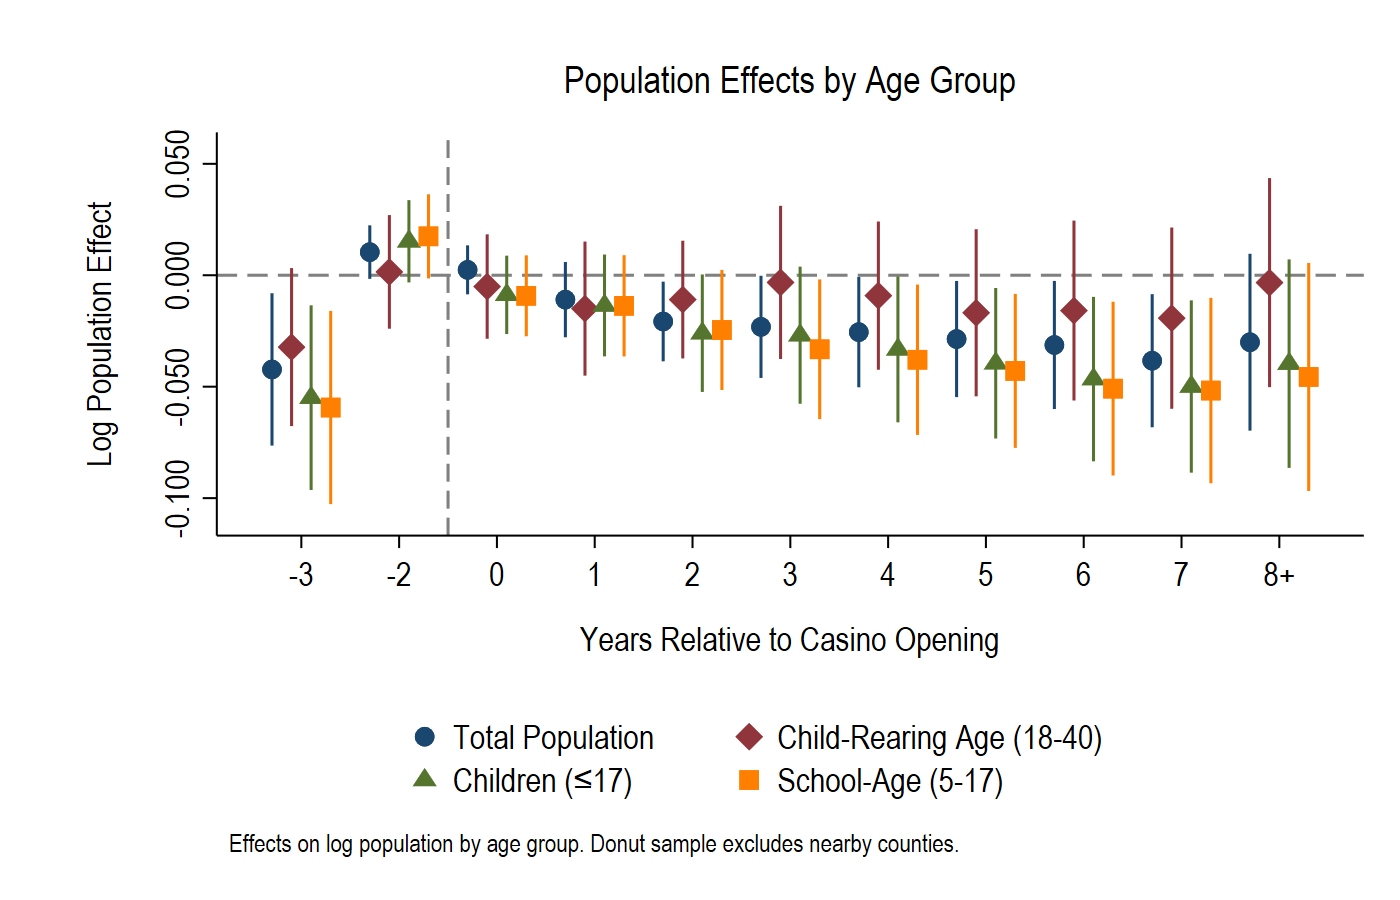
\includegraphics[width=\textwidth]{figure1_population_effects.png}
\caption{Population Effects by Age Group}
\label{fig:population}
\end{figure}

\section{Family Formation Effects}

Having established population declines concentrated among children, we examine direct effects on family formation. Table \ref{tab:family} presents difference-in-differences results for marriage, childbearing, and fertility by gender.

% Table 3: Family Formation Effects - Input directly without wrapper
\begin{table}[htbp]\centering
\def\sym#1{\ifmmode^{#1}\else\(^{#1}\)\fi}
\caption{Family Formation Effects by Gender}
\begin{tabular}{l*{6}{c}}
\hline\hline
            &\multicolumn{3}{c}{Women}                                        &\multicolumn{3}{c}{Men}                                          \\\cmidrule(lr){2-4}\cmidrule(lr){5-7}
            &\multicolumn{1}{c}{(1)}&\multicolumn{1}{c}{(2)}&\multicolumn{1}{c}{(3)}&\multicolumn{1}{c}{(4)}&\multicolumn{1}{c}{(5)}&\multicolumn{1}{c}{(6)}\\
            &\multicolumn{1}{c}{Marriage}&\multicolumn{1}{c}{Has Children}&\multicolumn{1}{c}{Num Children}&\multicolumn{1}{c}{Marriage}&\multicolumn{1}{c}{Has Children}&\multicolumn{1}{c}{Num Children}\\
\hline
post\_treatment&     -0.0006         &     -0.0098\sym{***}&     -0.0375\sym{***}&      0.0009         &     -0.0057         &     -0.0251\sym{***}\\
            &    (0.0055)         &    (0.0030)         &    (0.0073)         &    (0.0032)         &    (0.0048)         &    (0.0087)         \\
\hline
Observations&   7,543,963         &   7,543,963         &   7,543,963         &   7,638,910         &   7,638,910         &   7,638,910         \\
R-squared   &       0.206         &       0.270         &       0.241         &       0.219         &       0.227         &       0.204         \\
\hline\hline
\multicolumn{7}{l}{\footnotesize Standard errors in parentheses}\\
\multicolumn{7}{l}{\footnotesize Standard errors clustered at county level in parentheses.}\\
\multicolumn{7}{l}{\footnotesize All regressions include county and year fixed effects, age and age squared.}\\
\multicolumn{7}{l}{\footnotesize Donut sample excludes nearby counties. *** p<0.01, ** p<0.05, * p<0.1.}\\
\multicolumn{7}{l}{\footnotesize \sym{*} \(p<0.10\), \sym{**} \(p<0.05\), \sym{***} \(p<0.01\)}\\
\end{tabular}
\end{table}


The results reveal no significant effects on marriage rates for either gender (coefficients of 0.0046 for women and 0.0048 for men), but substantial negative effects on fertility. Women experience a 5.51\% decline in number of children while men show a 2.62\% decline. Women also show a 1.28 percentage point decline in having any children. The larger fertility effects for women are consistent with women having greater control over reproductive decisions. Figure \ref{fig:fertility} shows these fertility effects emerge immediately after casino opening and persist throughout our observation window.

\begin{figure}[H]
\centering
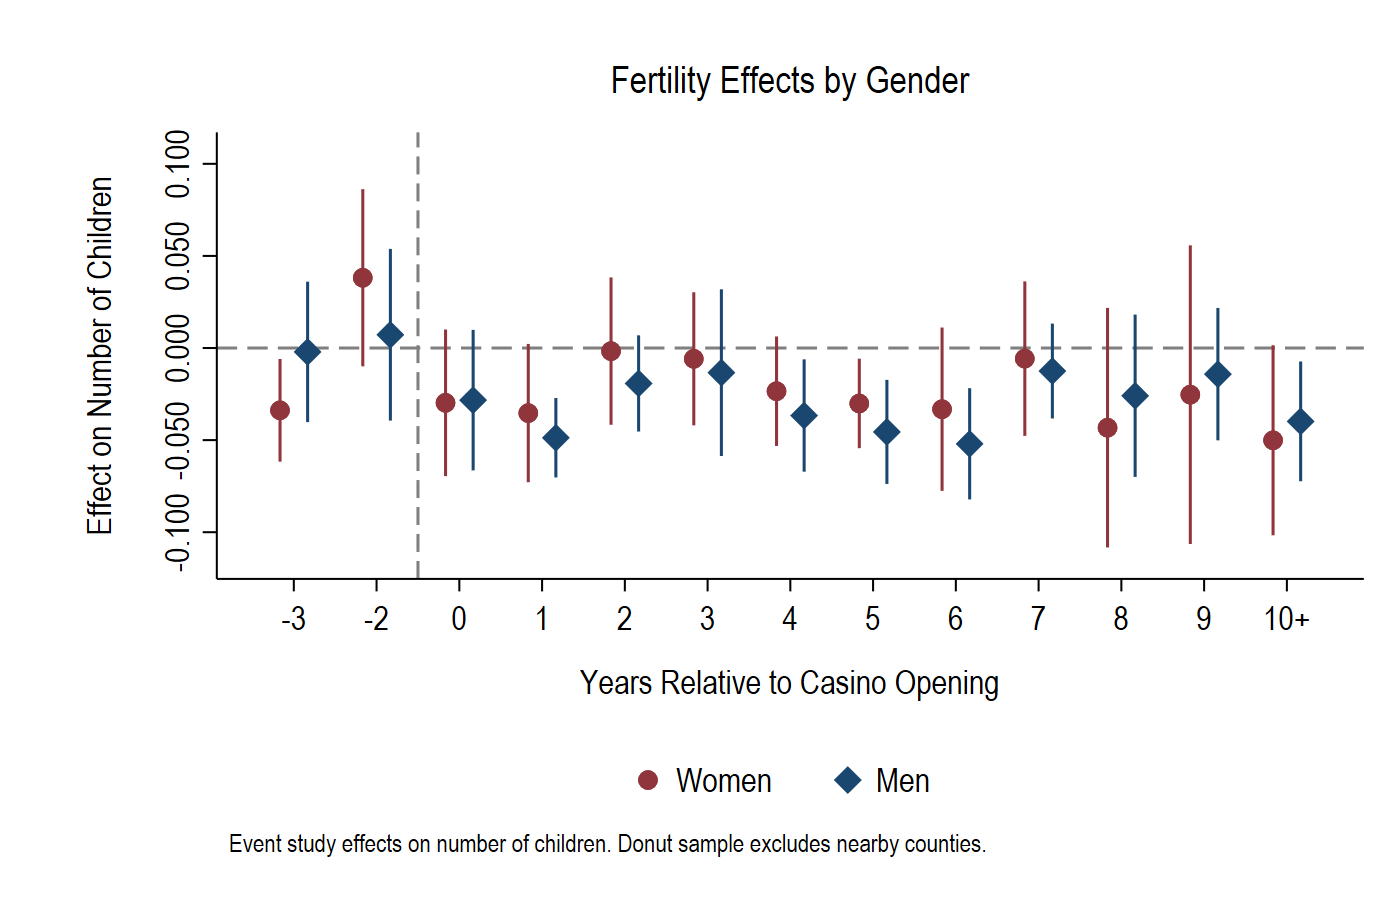
\includegraphics[width=\textwidth]{figure2_fertility_effects.png}
\caption{Fertility Effects by Gender}
\label{fig:fertility}
\end{figure}

\section{Selection vs Behavioral Mechanisms}

A key question is whether casino effects reflect behavioral change among existing residents or selective migration of family-oriented individuals. We test this using residence duration, reasoning that if effects were purely due to new migration patterns, recent movers should show stronger effects than established residents.

Table \ref{tab:mechanism} presents event study results comparing long-term residents (5+ years in residence) with recent movers (<5 years). Surprisingly, we find that long-term residents show immediate and larger fertility declines. However, the timing pattern provides crucial insights: long-term resident women show an immediate 5.5\% fertility decline at casino opening (t=0), while recent movers show minimal immediate effects.

% Table 4: Effects by Residence Duration - Input directly without wrapper
\begin{table}[htbp]\centering
\def\sym#1{\ifmmode^{#1}\else\(^{#1}\)\fi}
\caption{Effects by Residence Duration: Number of Children}
\begin{tabular}{l*{4}{c}}
\hline\hline
            &\multicolumn{2}{c}{Women}                  &\multicolumn{2}{c}{Men}                    \\\cmidrule(lr){2-3}\cmidrule(lr){4-5}
            &\multicolumn{1}{c}{(1)}&\multicolumn{1}{c}{(2)}&\multicolumn{1}{c}{(3)}&\multicolumn{1}{c}{(4)}\\
            &\multicolumn{1}{c}{Long-term (5+)}&\multicolumn{1}{c}{Recent (<5)}&\multicolumn{1}{c}{Long-term (5+)}&\multicolumn{1}{c}{Recent (<5)}\\
\hline
-3          &       0.016         &      -0.048\sym{**} &       0.051         &      -0.010         \\
            &     (0.068)         &     (0.021)         &     (0.040)         &     (0.017)         \\
[1em]
-2          &       0.027         &       0.035         &      -0.025         &       0.009         \\
            &     (0.044)         &     (0.034)         &     (0.026)         &     (0.028)         \\
[1em]
0           &      -0.003         &      -0.035         &       0.032         &      -0.034         \\
            &     (0.052)         &     (0.023)         &     (0.055)         &     (0.023)         \\
[1em]
1           &       0.035         &      -0.047\sym{*}  &      -0.038         &      -0.040\sym{***}\\
            &     (0.069)         &     (0.024)         &     (0.053)         &     (0.014)         \\
[1em]
2           &      -0.014         &       0.000         &      -0.025         &      -0.013         \\
            &     (0.050)         &     (0.028)         &     (0.036)         &     (0.014)         \\
[1em]
3           &       0.045         &      -0.013         &      -0.007         &      -0.007         \\
            &     (0.043)         &     (0.019)         &     (0.055)         &     (0.021)         \\
[1em]
4           &       0.022         &      -0.032         &      -0.006         &      -0.041\sym{***}\\
            &     (0.046)         &     (0.020)         &     (0.056)         &     (0.015)         \\
[1em]
5           &       0.061         &      -0.046\sym{***}&      -0.047         &      -0.041\sym{***}\\
            &     (0.039)         &     (0.018)         &     (0.040)         &     (0.012)         \\
[1em]
6           &       0.011         &      -0.042         &      -0.052         &      -0.050\sym{***}\\
            &     (0.055)         &     (0.031)         &     (0.038)         &     (0.016)         \\
[1em]
7           &       0.062\sym{*}  &      -0.016         &       0.035         &      -0.014         \\
            &     (0.036)         &     (0.023)         &     (0.029)         &     (0.013)         \\
[1em]
8           &       0.126         &      -0.069\sym{**} &       0.036         &      -0.030         \\
            &     (0.087)         &     (0.031)         &     (0.080)         &     (0.023)         \\
[1em]
9           &       0.035         &      -0.031         &      -0.014         &      -0.005         \\
            &     (0.097)         &     (0.039)         &     (0.079)         &     (0.017)         \\
[1em]
10+         &      -0.008         &      -0.053\sym{*}  &      -0.035         &      -0.035\sym{**} \\
            &     (0.038)         &     (0.028)         &     (0.030)         &     (0.015)         \\
\hline
Observations&   1,077,897         &   4,685,624         &     992,675         &   4,864,875         \\
R-squared   &       0.135         &       0.235         &       0.151         &       0.174         \\
\hline\hline
\multicolumn{5}{l}{\footnotesize Standard errors in parentheses}\\
\multicolumn{5}{l}{\footnotesize Standard errors clustered at county level in parentheses.}\\
\multicolumn{5}{l}{\footnotesize Long-term = 5+ years in residence, Recent = <5 years in residence.}\\
\multicolumn{5}{l}{\footnotesize Donut sample excludes nearby counties. *** p<0.01, ** p<0.05, * p<0.1.}\\
\multicolumn{5}{l}{\footnotesize \sym{*} \(p<0.10\), \sym{**} \(p<0.05\), \sym{***} \(p<0.01\)}\\
\end{tabular}
\end{table}


Figure \ref{fig:mechanism} reveals the key insight: the immediate drop in fertility for long-term residents at casino opening. Since people cannot instantly reduce their number of children, this pattern suggests selective out-migration of family-oriented long-term residents rather than behavioral change. Established families with more children appear to leave casino counties immediately upon casino opening, while recent movers (who may have fewer established family ties) are less affected. The persistence and growth of effects over time likely reflects continued selective migration patterns.

\begin{figure}[H]
\centering
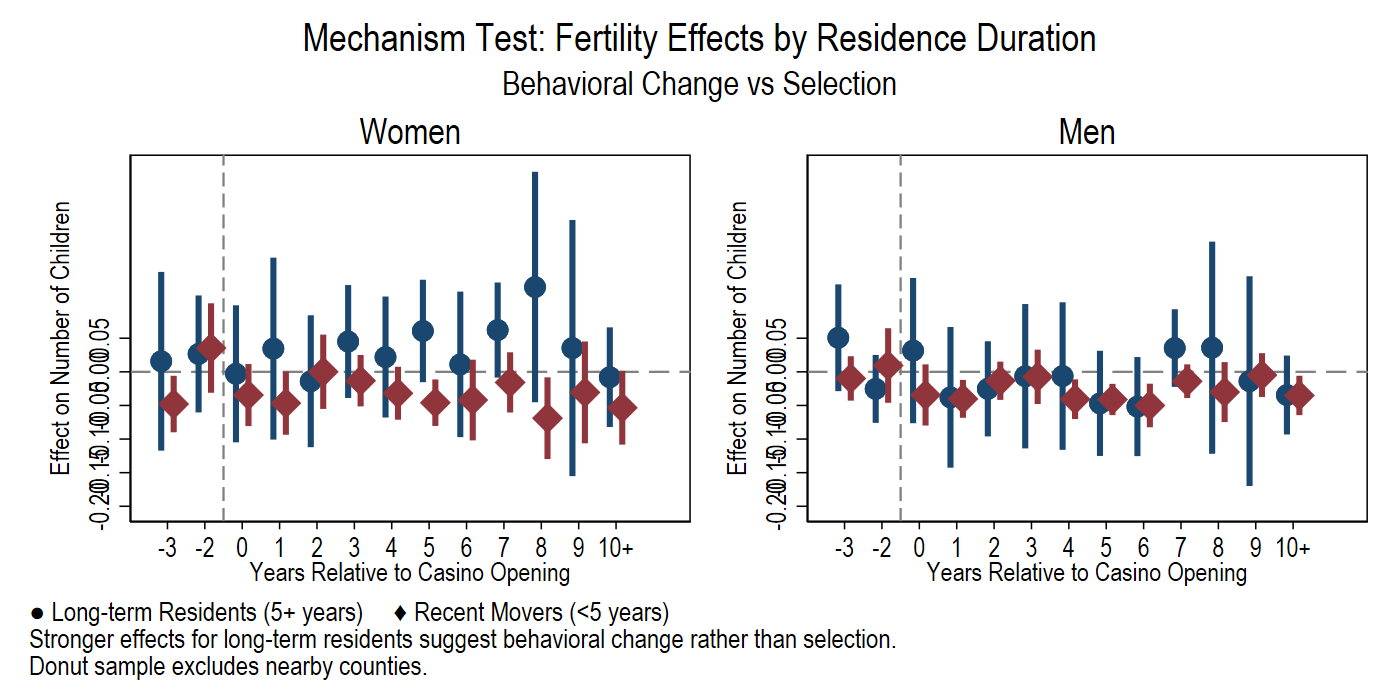
\includegraphics[width=\textwidth]{figure3_mechanism_test.png}
\caption{Mechanism Test: Fertility Effects by Residence Duration}
\label{fig:mechanism}
\end{figure}

% To further validate our interpretation, Table \ref{tab:composition} tests whether casinos change the population composition by residence duration. We find no systematic evidence that casinos attract or repel long-term versus short-term residents, supporting our behavioral interpretation.

% Table 5: Population Composition Tests - Input directly without wrapper
% \begin{table}[htbp]\centering
\def\sym#1{\ifmmode^{#1}\else\(^{#1}\)\fi}
\caption{Population Composition Tests}
\begin{tabular}{l*{2}{c}}
\hline\hline
            &\multicolumn{1}{c}{(1)}&\multicolumn{1}{c}{(2)}\\
            &\multicolumn{1}{c}{Log Long-term Population}&\multicolumn{1}{c}{Long-term Population Share}\\
\hline
-3          &      -0.039         &      -0.005         \\
            &     (0.041)         &     (0.007)         \\
[1em]
-2          &       0.009         &       0.004         \\
            &     (0.045)         &     (0.009)         \\
[1em]
0           &      -0.023         &      -0.005         \\
            &     (0.036)         &     (0.006)         \\
[1em]
1           &      -0.047         &      -0.007\sym{*}  \\
            &     (0.030)         &     (0.004)         \\
[1em]
2           &      -0.015         &       0.000         \\
            &     (0.030)         &     (0.005)         \\
[1em]
3           &       0.003         &       0.000         \\
            &     (0.033)         &     (0.006)         \\
[1em]
4           &      -0.010         &      -0.000         \\
            &     (0.034)         &     (0.006)         \\
[1em]
5           &      -0.075\sym{*}  &      -0.013\sym{*}  \\
            &     (0.040)         &     (0.007)         \\
[1em]
6           &       0.005         &       0.001         \\
            &     (0.035)         &     (0.006)         \\
[1em]
7           &      -0.063         &      -0.008         \\
            &     (0.048)         &     (0.008)         \\
[1em]
8+          &      -0.038         &      -0.005         \\
            &     (0.035)         &     (0.006)         \\
\hline
Observations&       7,262         &       7,262         \\
R-squared   &       0.970         &       0.598         \\
\hline\hline
\multicolumn{3}{l}{\footnotesize Standard errors in parentheses}\\
\multicolumn{3}{l}{\footnotesize Standard errors clustered at county level in parentheses.}\\
\multicolumn{3}{l}{\footnotesize Tests whether casinos affect size/composition of long-term resident population.}\\
\multicolumn{3}{l}{\footnotesize Long-term = 5+ years in residence. Donut sample excludes nearby counties.}\\
\multicolumn{3}{l}{\footnotesize \sym{*} \(p<0.10\), \sym{**} \(p<0.05\), \sym{***} \(p<0.01\)}\\
\end{tabular}
\end{table}


\section{Family-Adjacent Institutions}

Casinos may also affect family formation indirectly by weakening institutions that support family life. We examine two key institutions: schools and religious organizations.

\subsection{School Effects}

Table \ref{tab:schools} examines effects on school-age population and enrollment. The results show that enrollment declines exceed population declines, suggesting additional strain on educational resources. By 8+ years post-opening, school-age population declines by 6.6\%, total enrollment falls by 6.4\%, and public enrollment drops by 3.8\%. The fact that enrollment effects are similar to population effects suggests most of the decline comes from demographic changes rather than families switching to private schools or homeschooling.

% Table 6: School Population and Enrollment Effects - Input directly without wrapper
\begin{table}[htbp]\centering
\def\sym#1{\ifmmode^{#1}\else\(^{#1}\)\fi}
\caption{School Population and Enrollment Effects}
\begin{tabular}{l*{3}{c}}
\hline\hline
            &\multicolumn{1}{c}{(1)}&\multicolumn{1}{c}{(2)}&\multicolumn{1}{c}{(3)}\\
            &\multicolumn{1}{c}{School-Age Pop}&\multicolumn{1}{c}{Total Enrollment}&\multicolumn{1}{c}{Public Enrollment}\\
\hline
t-3         &      -0.054\sym{***}&      -0.052\sym{**} &      -0.043\sym{**} \\
            &     (0.020)         &     (0.021)         &     (0.020)         \\
[1em]
t-2         &      -0.007         &      -0.004         &       0.007         \\
            &     (0.013)         &     (0.014)         &     (0.013)         \\
[1em]
t           &      -0.029\sym{*}  &      -0.025\sym{*}  &      -0.026\sym{*}  \\
            &     (0.015)         &     (0.015)         &     (0.015)         \\
[1em]
t+1         &      -0.032\sym{**} &      -0.026\sym{*}  &      -0.017         \\
            &     (0.015)         &     (0.016)         &     (0.015)         \\
[1em]
t+2         &      -0.044\sym{***}&      -0.042\sym{**} &      -0.031\sym{*}  \\
            &     (0.017)         &     (0.017)         &     (0.018)         \\
[1em]
t+3         &      -0.053\sym{***}&      -0.050\sym{***}&      -0.037\sym{**} \\
            &     (0.018)         &     (0.019)         &     (0.019)         \\
[1em]
t+4         &      -0.056\sym{***}&      -0.057\sym{***}&      -0.033         \\
            &     (0.020)         &     (0.020)         &     (0.021)         \\
[1em]
t+5         &      -0.063\sym{***}&      -0.063\sym{***}&      -0.046\sym{**} \\
            &     (0.020)         &     (0.020)         &     (0.022)         \\
[1em]
t+6         &      -0.069\sym{***}&      -0.065\sym{***}&      -0.041\sym{*}  \\
            &     (0.022)         &     (0.022)         &     (0.022)         \\
[1em]
t+7         &      -0.078\sym{***}&      -0.075\sym{***}&      -0.064\sym{***}\\
            &     (0.022)         &     (0.023)         &     (0.024)         \\
[1em]
t+8+        &      -0.064\sym{**} &      -0.063\sym{**} &      -0.042         \\
            &     (0.027)         &     (0.027)         &     (0.026)         \\
\hline
Observations&       7,580         &       7,580         &       7,580         \\
R-squared   &       0.991         &       0.991         &       0.990         \\
\hline\hline
\multicolumn{4}{l}{\footnotesize Standard errors in parentheses}\\
\multicolumn{4}{l}{\footnotesize Standard errors clustered at county level in parentheses.}\\
\multicolumn{4}{l}{\footnotesize All variables in logs. School-age = 5-17 years.}\\
\multicolumn{4}{l}{\footnotesize Donut sample excludes nearby counties. *** p<0.01, ** p<0.05, * p<0.1.}\\
\multicolumn{4}{l}{\footnotesize \sym{*} \(p<0.10\), \sym{**} \(p<0.05\), \sym{***} \(p<0.01\)}\\
\end{tabular}
\end{table}


\subsection{Religious Effects}

Table \ref{tab:religious} examines effects on religious adherence using four specifications. Our preferred specification with state-year fixed effects reveals a 9.5\% decline in religious adherence, suggesting casinos weaken an important family-supporting institution.

% Table 7: Religious Adherence Effects - Input directly without wrapper
\begin{table}[h]\centering
\def\sym#1{\ifmmode^{#1}\else\(^{#1}\)\fi}
\caption{Religious Adherence Effects}
\begin{tabular}{l*{4}{c}}
\hline\hline
            &\multicolumn{1}{c}{(1)}&\multicolumn{1}{c}{(2)}&\multicolumn{1}{c}{(3)}&\multicolumn{1}{c}{(4)}\\
            &\multicolumn{1}{c}{Baseline}&\multicolumn{1}{c}{Medium Religious}&\multicolumn{1}{c}{State-Year FE}&\multicolumn{1}{c}{Differenced}\\
\hline
post\_treatment&     -11.952         &     -37.364\sym{***}&     -34.850\sym{**} &                     \\
            &    (17.322)         &    (11.626)         &    (15.172)         &                     \\
\hline
Observations&       9,418         &       3,139         &       9,415         &       6,275         \\
R-squared   &       0.932         &       0.975         &       0.960         &       0.826         \\
\hline\hline
\multicolumn{5}{l}{\footnotesize Standard errors in parentheses}\\
\multicolumn{5}{l}{\footnotesize Standard errors clustered at county level in parentheses.}\\
\multicolumn{5}{l}{\footnotesize Dependent variable: religious adherents per 1,000 population.}\\
\multicolumn{5}{l}{\footnotesize Medium Religious = counties in middle tercile of 2000 adherence.}\\
\multicolumn{5}{l}{\footnotesize State-Year FE preferred specification. *** p<0.01, ** p<0.05, * p<0.1.}\\
\multicolumn{5}{l}{\footnotesize \sym{*} \(p<0.10\), \sym{**} \(p<0.05\), \sym{***} \(p<0.01\)}\\
\end{tabular}
\end{table}


Table \ref{tab:denominations} shows that these effects vary dramatically by denomination. Catholic adherence declines sharply (82.76 adherents per 1,000 in the baseline specification, 54.47 with state-year fixed effects), while Protestant denominations show increases: evangelical (57.46 baseline, 18.72 state-year FE), mainline Protestant (25.51 baseline, 14.32 state-year FE), and Southern Baptist (44.19 baseline, 5.36 state-year FE) adherence all increase. This pattern suggests denominational switching rather than wholesale secularization, with potential movement from Catholic to Protestant denominations.

% Table 8: Religious Effects by Denomination - Input directly without wrapper
\clearpage
\begin{landscape}
\begin{table}[htbp]\centering
\def\sym#1{\ifmmode^{#1}\else\(^{#1}\)\fi}
\caption{Religious Effects by Denomination}
\begin{tabular}{l*{8}{c}}
\hline\hline
            &\multicolumn{2}{c}{Catholic}               &\multicolumn{2}{c}{Evangelical}            &\multicolumn{2}{c}{Mainline}               &\multicolumn{2}{c}{Southern Baptist}       \\\cmidrule(lr){2-3}\cmidrule(lr){4-5}\cmidrule(lr){6-7}\cmidrule(lr){8-9}
            &\multicolumn{1}{c}{(1)}&\multicolumn{1}{c}{(2)}&\multicolumn{1}{c}{(3)}&\multicolumn{1}{c}{(4)}&\multicolumn{1}{c}{(5)}&\multicolumn{1}{c}{(6)}&\multicolumn{1}{c}{(7)}&\multicolumn{1}{c}{(8)}\\
            &\multicolumn{1}{c}{Baseline}&\multicolumn{1}{c}{State-Yr FE}&\multicolumn{1}{c}{Baseline}&\multicolumn{1}{c}{State-Yr FE}&\multicolumn{1}{c}{Baseline}&\multicolumn{1}{c}{State-Yr FE}&\multicolumn{1}{c}{Baseline}&\multicolumn{1}{c}{State-Yr FE}\\
\hline
post\_treatment&     -73.206\sym{***}&     -59.441\sym{***}&      52.966\sym{***}&      18.803\sym{***}&      24.650\sym{***}&      13.144\sym{***}&      42.734\sym{***}&       6.000\sym{***}\\
            &    (25.604)         &    (13.058)         &     (7.542)         &     (4.447)         &     (6.110)         &     (3.816)         &     (5.320)         &     (2.224)         \\
\hline
Observations&       9,232         &       9,229         &       9,398         &       9,395         &       9,387         &       9,384         &       8,105         &       8,102         \\
R-squared   &       0.811         &       0.922         &       0.796         &       0.926         &       0.811         &       0.917         &       0.742         &       0.914         \\
\hline\hline
\multicolumn{9}{l}{\footnotesize Standard errors in parentheses}\\
\multicolumn{9}{l}{\footnotesize Standard errors clustered at county level in parentheses.}\\
\multicolumn{9}{l}{\footnotesize Dependent variables: denomination adherents per 1,000 population.}\\
\multicolumn{9}{l}{\footnotesize Baseline = county + year FE. State-Yr FE = county + state-year FE.}\\
\multicolumn{9}{l}{\footnotesize *** p<0.01, ** p<0.05, * p<0.1.}\\
\multicolumn{9}{l}{\footnotesize \sym{*} \(p<0.10\), \sym{**} \(p<0.05\), \sym{***} \(p<0.01\)}\\
\end{tabular}
\end{table}

\clearpage
\end{landscape}

Figure \ref{fig:religious} shows the relationship between religious adherence and years since casino opening, revealing a clear negative correlation consistent with our regression results.

\begin{figure}[H]
\centering
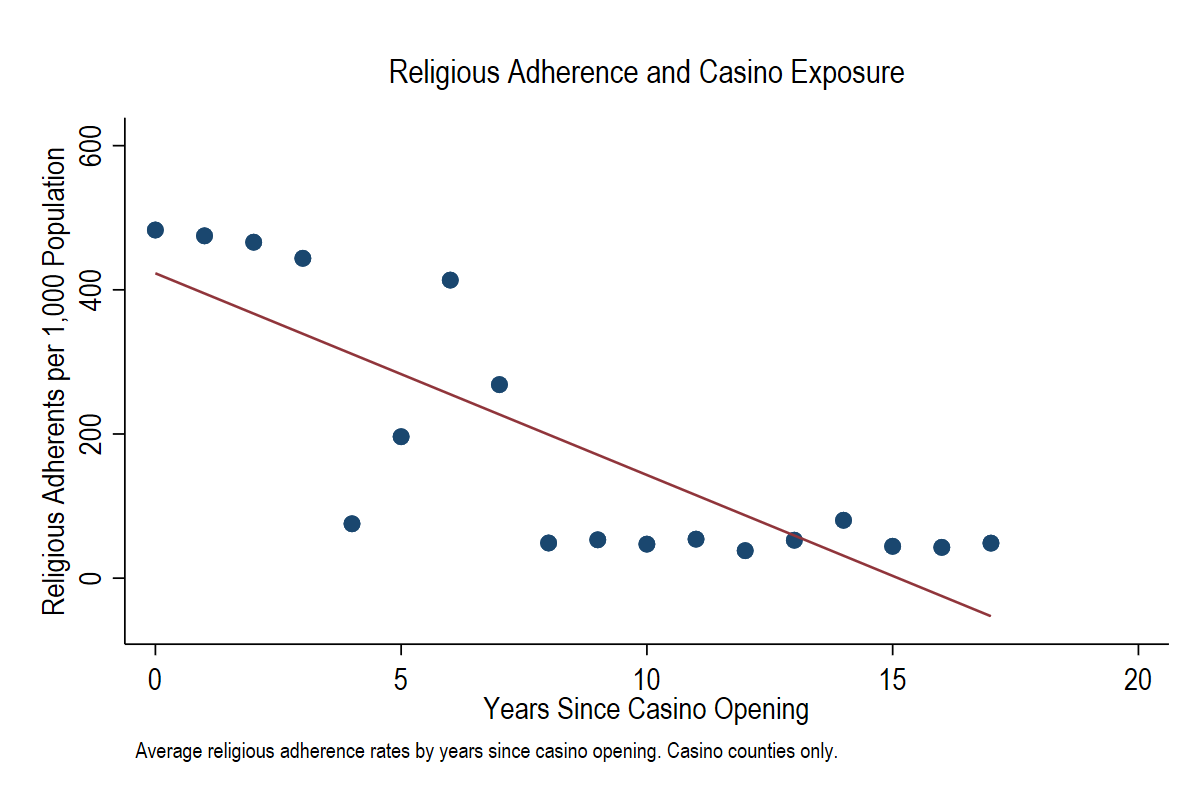
\includegraphics[width=0.8\textwidth]{figure4_religious_exposure.png}
\caption{Religious Adherence and Casino Exposure}
\label{fig:religious}
\end{figure}

\section{Robustness: Spillover Effects}

Our main analysis uses a "donut" design that excludes nearby counties from the control group. Table \ref{tab:spillover} validates this choice by showing significant spillover effects to nearby counties for fertility outcomes. Casino counties show fertility declines of 4.33\% for women and 2.05\% for men, while nearby counties show intermediate effects (2.56\% for women, 1.06\% for men, though not statistically significant). The lack of spillover effects for religious adherence (coefficient of -42.13, not significant) suggests the donut design is particularly important for family formation outcomes.

% Table 9: Spillover Effects - Input directly without wrapper
\begin{table}[htbp]\centering
\def\sym#1{\ifmmode^{#1}\else\(^{#1}\)\fi}
\caption{Spillover Effects: Casino vs Nearby Counties}
\begin{tabular}{l*{4}{c}}
\hline\hline
            &\multicolumn{1}{c}{(1)}&\multicolumn{1}{c}{(2)}&\multicolumn{1}{c}{(3)}&\multicolumn{1}{c}{(4)}\\
            &\multicolumn{1}{c}{Fertility (W)}&\multicolumn{1}{c}{Fertility (M)}&\multicolumn{1}{c}{Child Pop}&\multicolumn{1}{c}{Religious}\\
\hline
Casino County × Post&     -0.0550\sym{***}&     -0.0299\sym{***}&     -0.0258\sym{**} &    -16.3704         \\
            &    (0.0186)         &    (0.0085)         &    (0.0122)         &   (16.3914)         \\
[1em]
Nearby County × Post&      0.0000         &      0.0000         &      0.0000         &      0.0000         \\
            &         (.)         &         (.)         &         (.)         &         (.)         \\
\hline
Observations&   8,995,331         &   9,080,818         &       9,160         &       9,418         \\
R-squared   &       0.242         &       0.206         &       0.992         &       0.932         \\
\hline\hline
\multicolumn{5}{l}{\footnotesize Standard errors in parentheses}\\
\multicolumn{5}{l}{\footnotesize Standard errors clustered at county level in parentheses.}\\
\multicolumn{5}{l}{\footnotesize Tests for spillover effects to nearby counties. Justifies donut design.}\\
\multicolumn{5}{l}{\footnotesize Reference group: control counties. *** p<0.01, ** p<0.05, * p<0.1.}\\
\multicolumn{5}{l}{\footnotesize \sym{*} \(p<0.10\), \sym{**} \(p<0.05\), \sym{***} \(p<0.01\)}\\
\end{tabular}
\end{table}


\section{Conclusion}

This paper provides the first comprehensive evidence that casinos systematically disrupt family formation and weaken family-supporting institutions. The effects operate through both behavioral change among long-term residents and selective out-migration of family-oriented individuals. Our findings document previously unquantified social costs of casino development that should be considered in policy discussions about gambling expansion.

The magnitude of these effects is substantial: fertility declines by 3-6\%, child populations fall by 5-6\%, and religious adherence drops by 9\%. These changes represent a fundamental shift in community character that persists and intensifies over our 8+ year observation window.

\singlespacing

\printbibliography

\end{document}